\documentclass [11pt, a4wide, twoside]{article}

\usepackage{times}
\usepackage{epsfig}
\usepackage{ifthen}
\usepackage{xspace}
\usepackage{fancyhdr}
\usepackage[colorlinks,urlcolor=blue]{hyperref}
\usepackage{verbatim}
\usepackage{graphicx} 

\usepackage{listings}
\usepackage{color}

\definecolor{dkgreen}{rgb}{0,0.6,0}
\definecolor{gray}{rgb}{0.5,0.5,0.5}
\definecolor{mauve}{rgb}{0.58,0,0.82}

\lstset{frame=tb,
  language=Java,
  aboveskip=3mm,
  belowskip=3mm,
  showstringspaces=false,
  columns=flexible,
  basicstyle={\fontfamily{pcr}\selectfont},
  numbers=none,
  numberstyle=\tiny\color{gray},
  keywordstyle=\color{blue},
  commentstyle=\color{dkgreen},
  stringstyle=\color{mauve},
  breaklines=true,
  breakatwhitespace=true,
  tabsize=3
}

\graphicspath{{.}}

% solution switch
\newboolean{showsolution}
\setboolean{showsolution}{true} 

\usepackage{times}
\usepackage{epsfig}
\usepackage{ifthen}
\usepackage{xspace}
\usepackage{fancyhdr}
\usepackage{amsthm}
\usepackage{hyperref}



%layout
\topmargin      -5.0mm
\oddsidemargin  6.0mm
\evensidemargin -6.0mm
\textheight     215.5mm
\textwidth      160.0mm
\parindent      1.0em
\headsep        10.3mm
\headheight     12pt
\lineskip       1pt
\normallineskip 1pt

\newtheorem{mydef}{Definition}


%header
\lhead{Software Modeling and Analysis \\ 2016}

\rhead{Prof. Oscar Nierstrasz, Mohammad Ghafari, Nevena Milojkovi\'{c} and Yuriy Tymchuk}

\lfoot{page \thepage}
\rfoot{\today}
\cfoot{}

\renewcommand{\headrulewidth}{0.1pt}
\renewcommand{\footrulewidth}{0.1pt}

%enumeration
\newenvironment{myitemize}{%
     \begin{itemize}
     \setlength{\itemsep}{0cm}}
     {\end{itemize}}

\newenvironment{myenumerate}{%
     \begin{enumerate} \setlength{\itemsep}{0cm}}
     {\end{enumerate}}


%solution
\ifthenelse{\boolean{showsolution}}
   {  \newcommand{\solution}[1]{
   	\noindent\underline{\textbf{Answer:}}\\[2mm]
   	 \textsl{#1}
	 \vspace{10pt}
	 \normalsize
	}
  }
  {  \newcommand{\solution}[1]{} }


\pagestyle{fancy}

% ============================================================
% Markup macros for proof-reading
\usepackage{ifthen}
\usepackage[normalem]{ulem} % for \sout
\usepackage{xcolor}
\newcommand{\ra}{$\rightarrow$}
\newboolean{showedits}
\setboolean{showedits}{true} % toggle to show or hide edits
\ifthenelse{\boolean{showedits}}
{
	\newcommand{\ugh}[1]{\textcolor{red}{\uwave{#1}}} % please rephrase
	\newcommand{\ins}[1]{\textcolor{blue}{\uline{#1}}} % please insert
	\newcommand{\del}[1]{\textcolor{red}{\sout{#1}}} % please delete
	\newcommand{\chg}[2]{\textcolor{red}{\sout{#1}}{\ra}\textcolor{blue}{\uline{#2}}} % please change
}{
	\newcommand{\ugh}[1]{#1} % please rephrase
	\newcommand{\ins}[1]{#1} % please insert
	\newcommand{\del}[1]{} % please delete
	\newcommand{\chg}[2]{#2}
}
% ============================================================
% Put edit comments in a really ugly standout display
%\usepackage{ifthen}
\usepackage{amssymb}
\newboolean{showcomments}
\setboolean{showcomments}{true}
%\setboolean{showcomments}{false}
\newcommand{\id}[1]{$-$Id: scgPaper.tex 32478 2010-04-29 09:11:32Z oscar $-$}
\newcommand{\yellowbox}[1]{\fcolorbox{gray}{yellow}{\bfseries\sffamily\scriptsize#1}}
\newcommand{\triangles}[1]{{\sf\small$\blacktriangleright$\textit{#1}$\blacktriangleleft$}}
\ifthenelse{\boolean{showcomments}}
%{\newcommand{\nb}[2]{{\yellowbox{#1}\triangles{#2}}}
{\newcommand{\nbc}[3]{
 {\colorbox{#3}{\bfseries\sffamily\scriptsize\textcolor{white}{#1}}}
 {\textcolor{#3}{\sf\small$\blacktriangleright$\textit{#2}$\blacktriangleleft$}}}
 \newcommand{\version}{\emph{\scriptsize\id}}}
{\newcommand{\nbc}[3]{}
 \renewcommand{\ugh}[1]{#1} % please rephrase
 \renewcommand{\ins}[1]{#1} % please insert
 \renewcommand{\del}[1]{} % please delete
 \renewcommand{\chg}[2]{#2} % please change
 \newcommand{\version}{}}
\newcommand{\nb}[2]{\nbc{#1}{#2}{orange}}
\newcommand{\here}{\yellowbox{$\Rightarrow$ CONTINUE HERE $\Leftarrow$}}
\newcommand\rev[2]{\nb{TODO (rev #1)}{#2}} % reviewer comments
\newcommand\fix[1]{\nb{FIX}{#1}}
\newcommand\todo[1]{\nb{TO DO}{#1}}
\newcommand\on[1]{\nbc{ON}{#1}{red}} % add more author macros here
%\newcommand\XXX[1]{\nbc{XXX}{#1}{blue}}
%\newcommand\XXX[1]{\nbc{XXX}{#1}{brown}}
%\newcommand\XXX[1]{\nbc{XXX}{#1}{cyan}}
%\newcommand\XXX[1]{\nbc{XXX}{#1}{darkgray}}
%\newcommand\XXX[1]{\nbc{XXX}{#1}{gray}}
%\newcommand\XXX[1]{\nbc{XXX}{#1}{magenta}}
%\newcommand\XXX[1]{\nbc{XXX}{#1}{olive}}
%\newcommand\XXX[1]{\nbc{XXX}{#1}{orange}}
%\newcommand\XXX[1]{\nbc{XXX}{#1}{purple}}
%\newcommand\XXX[1]{\nbc{XXX}{#1}{red}}
%\newcommand\XXX[1]{\nbc{XXX}{#1}{teal}}
%\newcommand\XXX[1]{\nbc{XXX}{#1}{violet}}
%=============================================================
% ST80 listings macros
% Adapted from Squeak by Example book
%=============================================================
% If you want >>> appearing as right guillemet, you need these two lines:
%\usepackage[T1]{fontenc}
%\newcommand{\sep}{\mbox{>>}}
% Otherwise use this:
\newcommand{\sep}{\mbox{$\gg$}}
%=============================================================
%:\needlines{N} before code block to force page feed
\usepackage{needspace}
\newcommand{\needlines}[1]{\Needspace{#1\baselineskip}}
%=============================================================
%:Listings package configuration for ST80
\usepackage[english]{babel}
\usepackage{amssymb,textcomp}
\usepackage{listings}
% \usepackage[usenames,dvipsnames]{color}
% \usepackage[usenames]{color}
% \definecolor{source}{gray}{0.95}
\lstdefinelanguage{Smalltalk}{
%  morekeywords={self,super,true,false,nil,thisContext}, % This is overkill
  morestring=[d]',
  morecomment=[s]{"}{"},
  alsoletter={\#:},
  escapechar={!},
  literate=
    {BANG}{!}1
    {UNDERSCORE}{\_}1
    {\\st}{Smalltalk}9 % convenience -- in case \st occurs in code
    % {'}{{\textquotesingle}}1 % replaced by upquote=true in \lstset
    {_}{{$\leftarrow$}}1
    {>>>}{{\sep}}1
    {^}{{$\uparrow$}}1
    {~}{{$\sim$}}1
    {-}{{\sf -\hspace{-0.13em}-}}1  % the goal is to make - the same width as +
    {+}{\raisebox{0.08ex}{+}}1		% and to raise + off the baseline to match -
    {-->}{{\quad$\longrightarrow$\quad}}3
	, % Don't forget the comma at the end!
  tabsize=4
}[keywords,comments,strings]

\definecolor{source}{gray}{0.95}

\lstset{language=Smalltalk,
	basicstyle=\sffamily,
	keywordstyle=\color{black}\bfseries,
	% stringstyle=\ttfamily, % Ugly! do we really want this? -- on
	mathescape=true,
	showstringspaces=false,
	keepspaces=true,
	breaklines=true,
	breakautoindent=true,
	backgroundcolor=\color{source},
	lineskip={-1pt}, % Ugly hack
	upquote=true, % straight quote; requires textcomp package
	columns=fullflexible} % no fixed width fonts
% In-line code (literal)
% Normally use this for all in-line code:
\newcommand{\ct}{\lstinline[mathescape=false,backgroundcolor=\color{white},basicstyle={\sffamily\upshape}]}
% In-line code (latex enabled)
% Use this only in special situations where \ct does not work
% (within section headings ...):
\newcommand{\lct}[1]{{\textsf{\textup{#1}}}}
% Code environments
\lstnewenvironment{code}{%
	\lstset{%
		% frame=lines,
		frame=single,
		framerule=0pt,
		mathescape=false
	}
}{}

% Useful to add a matching $ after code containing a $
% \def\ignoredollar#1{}
%=============================================================
\newcommand{\ie}{\emph{i.e.}\xspace}
\newcommand{\eg}{\emph{e.g.}\xspace}
\newcommand{\etal}{\emph{et al.}\xspace}
% ============================================================


\begin{document}

\section*{\ifthenelse{\boolean{showsolution}}{\textcolor{red}{Solution}\\}{}Assignment 02  --- 23.09.2020 -- v1.0\\Smalltalk: A Reflective Language}

\textcolor{red}{Please submit this assignment by email to \href{mailto:pascal.gadient@inf.unibe.ch}{pascal.gadient@inf.unibe.ch} \underline{before} 30. September 2020, 10:15am.}\\

\noindent \textbf{For this assignment you have to download and install Glamorous Toolkit (GT) from \href{https://gtoolkit.com/}{here}.}

\subsection*{Exercise 1 - Nature of Smalltalk and GT (5 pts)}
\begin{enumerate}[a)]
\item What do you have to consider when you use a live system for software development? In other words, name one major threat that cannot arise in traditional software development, \eg with Java, C++, etc.?
\solution{Everything can be changed including system objects and language features. As a result, testing of random code might alter the execution environment and introduce future problems. For instance, your GT system will immediately crash if you randomly modify the code of kernel messages and classes, \eg you delete the \texttt{Object} class.}
\item What is a message in Smalltalk?
\solution{
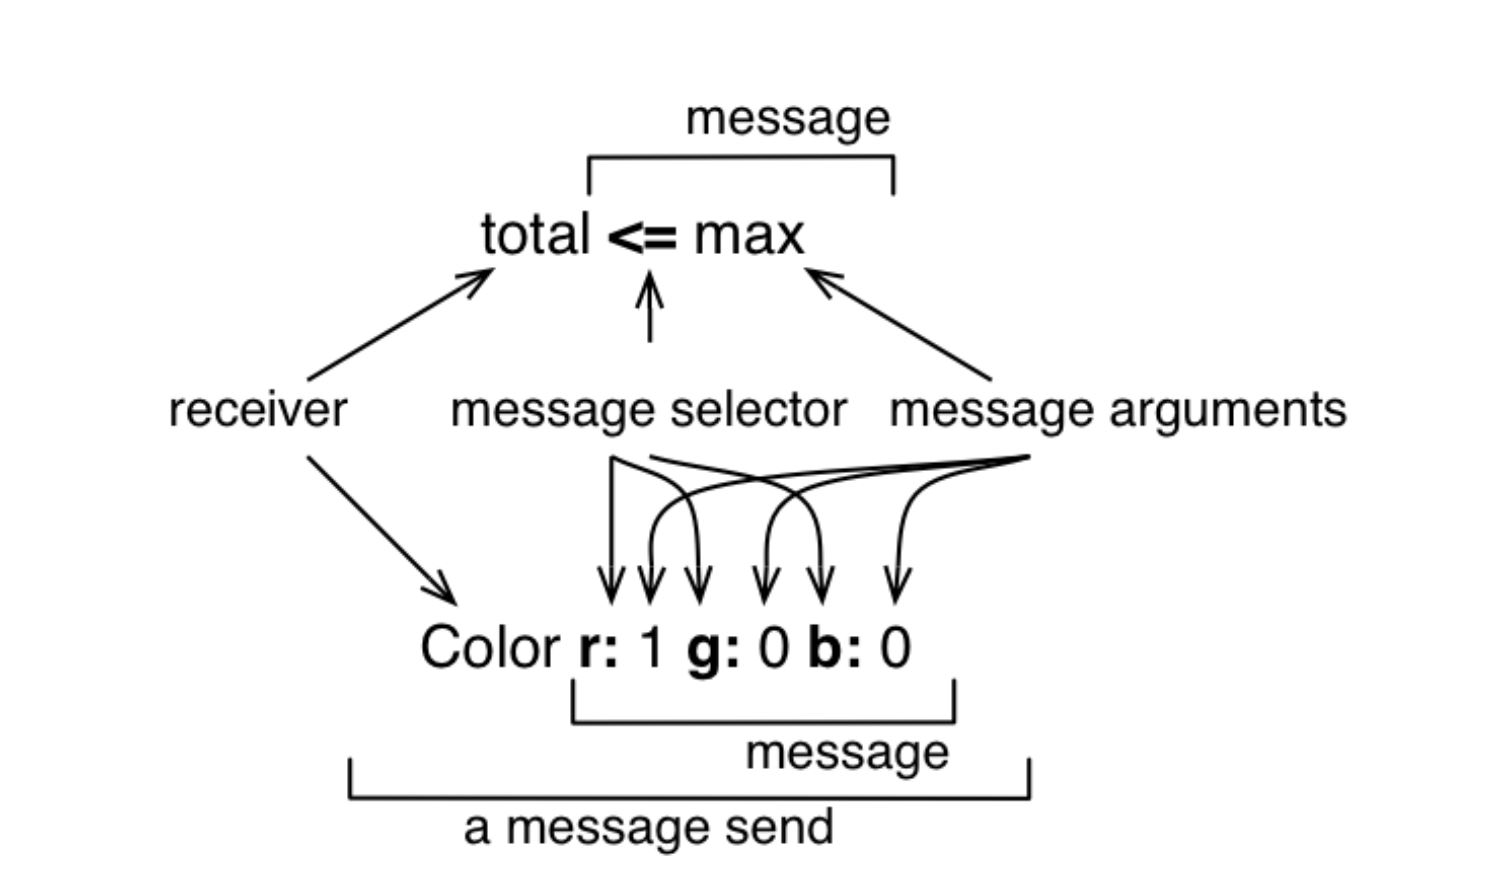
\includegraphics[scale=0.25]{message-definition}\\
All communication or interaction among objects is done by sending messages.
A message is composed of the message selector and the optional message arguments.
A message is sent to a receiver.
The combination of a message and its receiver is called a message send.}
\item What is a block in Smalltalk?
\solution{
A block can be thought of as a lambda-expression defining an anonymous function, or as a function object.
%A block is a piece of code whose execution is frozen and can be kicked in using messages.
%A block is a lambda expression or anonymous function that captures (or closes over) its environment at creation-time.
Square brackets \texttt{[ ]} define a block, also known as a block closure or a lexical closure, which is a first-class object representing a function.\\
Blocks may take one or more arguments (\texttt{[:i :j :k | ... ]}) and can have local variables.}
\item How do Smalltalk, Pharo, and GT relate to each other?
\solution{Smalltalk is the programming language used in Pharo and GT. Although the language stands on its own, it has many ties to its implementations in Pharo and GT that define the available instruction set (similar to libraries in other languages). Pharo is (mostly) implemented in Smalltalk. GT is a sophisticated framework written in Smalltalk on top of Pharo that uses a headless VM. GT tries to improve productivity and leverages many new features, \eg native window support and interactive notebooks.}
\item What are counterparts of GT tools (Playground, Coder, Git, Monitor, ExamplesExplorer, Transcript, Morphic World, Spotter) in your favorite development environment?
\solution{\vspace{-0.75cm}
\begin{itemize}
\item Playground: a sophisticated (text-based) Shell that has various inspection capabilities.
\item Coder: an integrated development environment (IDE) to edit existing packages, classes, and messages.
\item Git: a Git client.
\item Monitor: similar to a resource viewer (Linux, macOS) or a task-manager (Windows).
\item ExamplesExplorer: (offline) help resources, \eg documentation and demos.
\item Transcript: debug or console output window.
\item Morphic World: the base Pharo windowing system and IDE, enables low-level access to Smalltalk classes and instances. Compared to Java applications, it is somewhat similar to the Java JDK (including its system libraries) in combination with the VM.
\item Spotter: a search that inspects names and file content.
\newline
\end{itemize}
}
\end{enumerate}

\vspace{1.5cm}
\ifthenelse{\boolean{showsolution}}{}{\begin{center}\center{\large{\textit{\textbf{Please continue reading on the next page.}}}\newpage}\end{center}}

\subsection*{Exercise 2 - Object inspection (4 pts)}
\begin{enumerate}[a)]
\item Explain the difference between a \texttt{String} and a \texttt{Symbol} object in Smalltalk. Why is this differentiation important?\\
\emph{Hint: The execution of the code below will reveal differences.}
\lstset{basicstyle=\ttfamily}
\begin{lstlisting}
  ('HeySmalltalker') == 'HeySmalltalker'.
  ('HeySmalltalker') asSymbol == #HeySmalltalker.
  ('Hey','Smalltalker') == 'HeySmalltalker'.
  ('Hey','Smalltalker') asSymbol == #HeySmalltalker.
\end{lstlisting}
\solution{\vspace{-0.75cm}
\begin{itemize}
\item Symbols are immutable and unique.
Strings are mutable and not unique. 
%Symbols should never be mutated.
Consequently, multiple String objects with the value ``Hello'' can coexist, but only one Symbol object \#Hello can be initialized during run time.
Since Symbols are immutable, they should never be used when their value has to change over time.
The benefit of using Symbols is the performance gain due to less expensive value comparisons.
%Symbols are like Strings, in that they contain a sequence of characters. However, unlike a string, a literal symbol is guaranteed to be globally unique. This unique behavior helps in the lookup scenarios.
%Strings and Symbols are Collections and therefore support the usual Collection methods.
\item 
\texttt{(\textquotesingle HeySmalltalker\textquotesingle) == \textquotesingle HeySmalltalker\textquotesingle.}\\
\textit{Comparison of two Strings, expected to return true (note that the outcome depends on the VM implementation).}\\ \newline
\texttt{(\textquotesingle HeySmalltalker\textquotesingle) asSymbol == \#HeySmalltalker.}\\
\textit{Comparison of two Symbols, expected to return true.}\\ \newline
\texttt{(\textquotesingle Hey\textquotesingle,\textquotesingle Smalltalker\textquotesingle) == \textquotesingle HeySmalltalker\textquotesingle.}\\
\textit{Comparison of two (concatenated) Strings, expected to return false (note that the outcome depends on the VM implementation).}\\ \newline
\texttt{(\textquotesingle Hey\textquotesingle,\textquotesingle Smalltalker\textquotesingle) asSymbol == \#HeySmalltalker.}\\
\textit{Comparison of two (concatenated) Symbols, expected to return true.}\\ \newline
\end{itemize}
}
\item Write the equivalent of the following piece of code in Smalltalk as a block, and execute it with the values \textless38, 44\textgreater , \textless65, 48\textgreater, and \textless48, 48\textgreater.

\textit{Hint: Use the transcript tool (one line example below) as replacement for the \texttt{print} method.}\\
\texttt{Transcript show: \textquotesingle your output here\textquotesingle}

\lstset{basicstyle=\ttfamily}
\begin{lstlisting}
   	int scoreOfPlayerA, scoreOfPlayerB;
	if(scoreOfPlayerA > scoreOfPlayerB)
		print "Player A Won"	
	else if(scoreOfPlayerA < scoreOfPlayerB)
		print "Player B Won";
	else
		print "Match is declared as draw";
\end{lstlisting}
\solution{Please download the solution \href{http://scg.unibe.ch/download/lectures/sma-exercises/A02E02d.zip}{here}.}
\item How many classes in GT implement the message \texttt{includes: anObject}?\\How many messages in GT use that particular message?\\
\textit{Note: For this task, you are supposed to use a fresh and unaltered copy of GT with no changes of yours.}
\solution{In order to find the relevant classes and messages, you can use the Spotter tool, use CTRL+M/CMD+M (implementors) and CTRL+N/CMD+N (references), or you can perform this task programmatically (with code). There might exist minor differences depending on the version of the GT image you use, and the included elements in your search. 
We found 60 classes that implement the message, and more than four thousand messages that use it (\eg 4\,531 in the current Apple macOS GT build).}
\item Which message in GT can be sent to a class to find all its subclasses?
\solution {\texttt{subclasses}}
\end{enumerate}

\vspace{1.5cm}
\ifthenelse{\boolean{showsolution}}{}{\begin{center}\center{\large{\textit{\textbf{Please continue reading on the next page.}}}\newpage}\end{center}}

\subsection*{Exercise 3 - CallGraph (1 pt)}
Find the top ten most frequently invoked methods in the provided CallGraph representation.\\

\noindent In order to perform this exercise, you must (i) execute the statement below to retrieve the ``CallGraph Demo'' in GT, and (ii) you have to download the \texttt{Calls.txt} file from \href{http://scg.unibe.ch/download/lectures/sma-exercises/A02E03-CallGraph-Data.zip}{here} and store it in the same folder as the GT image file.\\

\noindent \texttt{Metacello new baseline: \textquotesingle SMAForGt\textquotesingle;\\
repository: \textquotesingle github://onierstrasz/sma-examples/src\textquotesingle; load.}\\

\noindent \textit{Hint 1: You can find some examples for accessing the CallGraph in the ``CallGraph Demo''.}\\\\
\noindent \textit{Hint 2: Don't forget to submit your code snippet \underline{and} your results.}\\\\
\solution{\texttt{cg := CallGraph fromFile: \textquotesingle Calls.txt\textquotesingle.\\
result := (cg methods sorted: [ :a :b  | a calls size \textgreater= b calls size]) first:10.}
\\\\
Result:\\
org.clapper.util.misc.LRUMap\$LRULinkedList.addToHead\\
org.clapper.util.misc.FileHashMap.checkValidity\\
org.clapper.util.misc.MultiIterator.checkIterator\\
org.clapper.util.misc.LRUMap.doPut\\
org.clapper.util.misc.LRUMap.clearTo\\
org.clapper.util.misc.LRUMap\$LRULinkedListEntry.setKeyValue\\
org.clapper.util.text.AbstractVariableSubstituter.legalVariableCharacter\\
org.clapper.util.misc.MultiValueMap.keySet\\
org.clapper.util.misc.MultiValueMap.put\\
org.clapper.util.misc.FileHashMap\$ValuesFile.getFile}

\end{document}
